\subsection{Pozicijos nustatymas naudojant mobilų telefoną}

Pirmas darbas apžvalgai yra \cite{willemsenconcept}, ``Concept for building a MEMS based indoor localization system''. Darbas pasiūlo galimos navigacinės sistemos prototipą, kuris remiasi inerciniais jutikliais. Kaip prototipo pagrindą buvo pasirinkit du mobilieji telefonai, kurie turi barometrą, pagreičio ir giroskopo jutiklį.

Darbas pradedamas prototipo pagrindo apžvalga, o konkrečiai nuo barometro. Barometras kaip matavimo įrenginys gali būti panaudotas pastato vidaus navigacijai, kurio pagalba galima nustatyti aukštą, kuriame yra stebimas objektas. Oro slėgis $p_i$ yra konvertuojamas į barometro aukščio formulę

\begin{equation}
    h_i = \Bigg( 1 - \sqrt[\leftroot{-2}\uproot{2}5.255]{ \frac{p_i}{1013.25} } \Bigg) \times \frac{288.15}{0.0065},
\end{equation}

Testavimo bazė buvo panaudotas \textit{HafenCity University} pastatas, kuris turėjo keturis aukštus. Duomenų surinkimo metu, jutiklis buvo perneštas per visus pastato aukštus su 4-3-2-1-1-2-3-4 seka. Rezultatai yra pateikiami \ref{fig:floor_detection_with_barometer_data} pavyzdyje.

\begin{figure}[H]
    \centering
    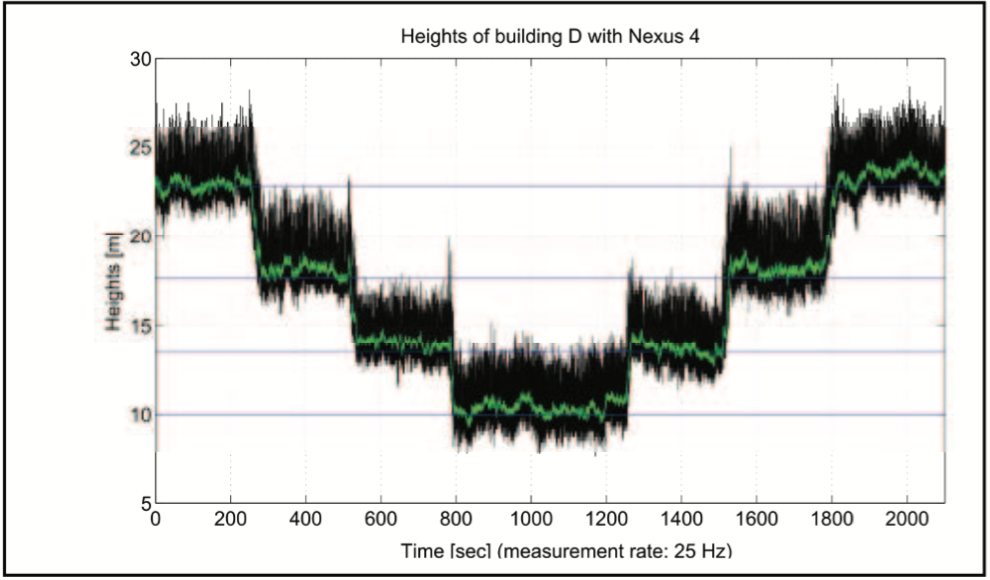
\includegraphics[width=300px]{img/floor_detection_with_barometer_data.png}
    \caption{Barometro naudojimas aukšto atpažinimui \cite{willemsenconcept}.}
    \label{fig:floor_detection_with_barometer_data}
\end{figure}

Grafike pavaizduotos juodos linijos vaizduoja gryną signalą, žalia juosta žymi vidutinį signalo įvertį per $1~s$ laikotarpį. Rezultatai labai ryškiai parodo, kad barometras gali būti panaudotas aukštui nustatyti.

Toliau yra nagrinėjamas pagreičio jutiklio pritaikymo galimybės. Iškarto yra teigiama, jog dviguba integracija, kuri gali būti panaudota apskaičiuojant nukeliautą atstumą yra visiškai negalimas panaudoti matmuo, kadangi pagreičio jutiklis yra labai linkęs dreifuoti. To pasekoje, jutiklis yra panaudojamas tik kaip žingsnių matuoklis. Žingsniui nustatyti yra panaudojamas sekantis metodas. Pirmiausiai yra laukiama kuomet pagreičio pokyčio vertė įkopia į teigiamą pusę. Tuomet algoritmas laukia neigiamo gradiento signale. Kai tik jis yra randamas -- detektuojamas žingsnis. Taip pat yra panaudojamas verčių buferis (angl. \textit{buffer}), norint minimizuoti klaidingą žingsnio radimą.

Kaip ir bet kokį jutiklį, pagreičio jutiklį reikia kalibruoti, nors iš pirmo žvilgsnio žingsnių atpažinimui to nereikia, tačiau būtent akselerometro pozicija nusako ašių gradientą, todėl norint tiksliai žinoti ašių etaloną, reikalinga kalibravimas. Tam autoriai vietinės srities gravitacijos įverčių duomenų bazę. Kalibravimo metodas yra paremtas \cite{wendel2011integrierte} Kalman filtru. Konteksto funkcija yra įgyvendinama per sferinį Pitagorą:

\begin{equation}
    g^2 = a_{xref}^2 + a_{yref}^2 + a_{zref}^2
\end{equation}

Santykis tarp atspirties (angl. \textit{reference}) vertės ir matavimo vertės, su pataisymu ir papildoma dedamąja yra išreiškiama

\begin{equation}
    a_{xref} = s_x (a_x + b_x)
\end{equation}

\begin{equation}
    a_{yref} = s_y (a_y + b_y)
\end{equation}

\begin{equation}
    a_{zref} = s_z (a_z + b_z)
\end{equation}

Funkcinis modelis gali būti parenkamas taip, jog mastelio $s$ ir dedamosios $b$ parametrai yra atitinkamai pataisomi.

Kalibravimui reikalingi parametrai yra randami pirmiausiai apverčiant prototipinį įrenginį porą kartų aplink savo matavimo ašis. To tikslas yra sujungti pagreičio jutiklio kiekvieną iš teigiamos ir neigiamos ašių su gravitacija. Labai svarbu yra užtikrinti, kad sukimas vyksta lygiai pagal jutiklio centrą, kad išvengti papildomų kalibravimo klaidų.

Sekantis įrenginys nagrinėjimui yra giroskopas ir jo sukimo pokytis. Orientacijos įvertis yra gaunamas paprasčiausiai integruojant sukimo pokytį. Toks integralas sudaro galimybei atsirasti dreifui. Dreifas yra didžiausias klaidos šaltinis pigiuose MEMS jutikliuose. Darbe yra pastebėta, jog kalibruoti giroskopą nėra būtina, bet labai svarbu yra identifikuoti dreifą prieš pradedant matavimus. Tokiu tikslius matavimo pradžioje giroskopas yra paliekamas ramybės būsenoje. Tai yra pasiekiama įrenginį prilaikant ant stalo. Dažniausiai tokiu atveju bus matoma tiesiog nuolatinė dedamoji, tačiau niekas negarantuoja stabilios nuolatinės dedamosios. Klaida gali kisti per laikotarpį, todėl pažymėtina yra atlikti papildomas korekcijas per matavimo laikotarpį.

Toliau yra pateikiamas pavyzdys su naudojama įranga, konkrečiai su Samsung Galaxy Nexus telefonu. Labai svarbi detalė yra automatinė nuolatinės dedamosios korekcija, kuri įrenginyje įvyksta po $8~s$. Tai yra vadina \textit{ZUPT} (angl. \textit{Zero velocity UPdaTe}). Korekcija įvykdoma tik tuomet, kai jutiklis nėra judinamas. 

Pereinama nuo pačių jutiklių duomenų prie duomenų apdorojimo. Jutiklių matmenų nuskaitymui yra panaudojamas kelio skaičiavimo metodas (angl. \textit{Dead Reckoning}). Navigacijos labui, kampo pokytis yra integruojamas, o pagreičio jutiklis yra panaudojamas tik žingsnio radimui. Turint informacijos apie žingsnio ilgį ir esamą kryptį, santykinė pozicija gali būti apibrėžta taikant vektorinę sudėtį (angl. \textit{polar appending}). Įvertinant triukšmą, kuri turi tiek pagreičio, tiek giroskopo jutikliai vien tik jų duomenimis pasikliauti nėra galima, todėl reikia įsivesti pagalbos metodiką, kuri supaprastinama iki filtro problemos. Tai labai padeda išspręsti dviejų stochastinių elementų duomenų sujungimą. Sprendimui atlikti yra parenkamas Kalman filtras. Taip pat į papildomą pagalbą yra pajungiamas ir žemėlapis, kurio pagalba galima filtruoti duomenis.

Prieš atiduodant pagreičio duomenis į Kalman filtrą, įverčiai yra vidurkinami per laiko vienetą, norint bent kažkiek sumažinti triukšmą. Kalman filtro aukščio parametras yra nustatomas tiesiogiai iš atmosferos slėgio, pagal barometro duomenis. Tam yra panaudojama formulė, kuri buvo aprašyta aukščiau. Pagreičio jutiklio duomenims pirmiausiai yra atliekamas plokštumos nustatymas. Jutiklis turi tris plokštumas, o norima navigacijos plokštuma yra dviejų dimensijų, todėl reikia pirmiausiai nustatyti ašių polinkį.

Toliau yra aprašoma žingsnio nustatymo metodika, kuri turi labai didelę įtaką objekto greičiui. Pradžioje yra laukiama vertės į teigiamų verčių ašį, o paskui neigiamo gradiento. Tokia veiksmų seka nusako žingsnio įvykį. Toliau seka žingsnio ilgio komponentė, kuri yra labai svarbi, kadangi greičio ir pozicijos skaičiavimams tai yra labai aktuali informacija. Blogas žingsnio ilgio parinkimas įvelia papildomų matavimo klaidų į sistemą. Prieš tai atliktuose darbuose \cite{kim2004step, goyal2011strap} buvo bandymas nustatyti automatiškai nusakyti žingsnio ilgį pagal pagreičio jutiklio dažnį, amplitudę ir žingsnio ypatybes, kaip pavyzdžiui bato dydis ir lytis. Remiantis aprašyta metodika, žingsnio ilgį galima nuspėti iki $10~\%$ tikslumu.

Rotacijos ir pagreičio santykis matavimo vektoriuje yra panaudojami kampo kitimo vektoriui išlyginti. Aukštis yra tiesiogiai koreguojamas pagal santykinį aukštį, gaunamą pagal barometro duomenis, o pradinės pozicijos taškas pagal greičio vidurkį iš žingsnio matuoklio duomenų. Mažinant dreifą dėl integracinio kampo pokyčio, duomenis iš giroskopo $z$ ašies yra atremiami į magmetometro azimuto ašį. Kalman filtras yra inicijuojamas pagal dabartinės pozicijos šiaurės ašį. Prieš filtro pradžią reikia rasti esamą kampo pokyčio nukrypimą, todėl reikia atlikti kalibracija, kuri vykdoma 6 sekundes.

Pozicijos filtravimas su Kalman filtru rezultatai yra pateikiami \ref{fig:pozition_estimation_with_parctile_filter_a} pav. Mėlyna linija pavyzdyje parodo rezultatą, kuomet Kalman filtras neturi papildomos informacijos apie sienų krypties informaciją, Raudona linija pažymi rezultatą, kuomet sienų pozicijos informacija yra pateikiama į Kalman filtrų parametrus.

Jutiklių duomenis yra paruošiami ne tik Kalman filtrui, tačiau ir dalelių filtrui. Pozicijos nustatymui dalelių filtras yra įgyvendinamas naudojant paskirstytą dalelių modelį ir jų santykinį balansą sekančiai didžiausią tikimybę turinčiai būsenai. Žinomų šablonų naudojimas leidžia labai sumažinti dalelių skaičių dalelių filtre. To pasekoje padidėja pozicijos skaičiavimo greitis. Tokio filtro struktūrą yra pateikiama \cite{willemsen2013kalibrierung}. Po pradinio dalelių paskirstymo, priklausomai nuo ėjimo greičio yra keičiamas dalelių paskirstymas procese, kuriam turi įtakos ėjimo greitis ir kryptis. Nagrinėjamu atveju, greitis ir kryptis turi labai didelį triukšmą.

Dalelių filtro rezultatas yra pateikiamas \ref{fig:pozition_estimation_with_parctile_filter_b}. Duomenis yra panaudoti tokie patys, kaip ir Kalman filtro atveju. Raudonai pažymėti taškai pažymi labiausiai tikėtiną poziciją. Mėlyni ir juodi taškai yra apskaičiuojamoji pozicija. Pavyzdyje galima aiškiai pamatyti, kaip sienų pozicijos informacija eksperimento metu padarė įtaka objekto pozicijos skaičiavimams.

\begin{figure}[H]
    \label{fig:pozition_estimation_with_parctile_filter}
    \centering
    \subfloat[a][]{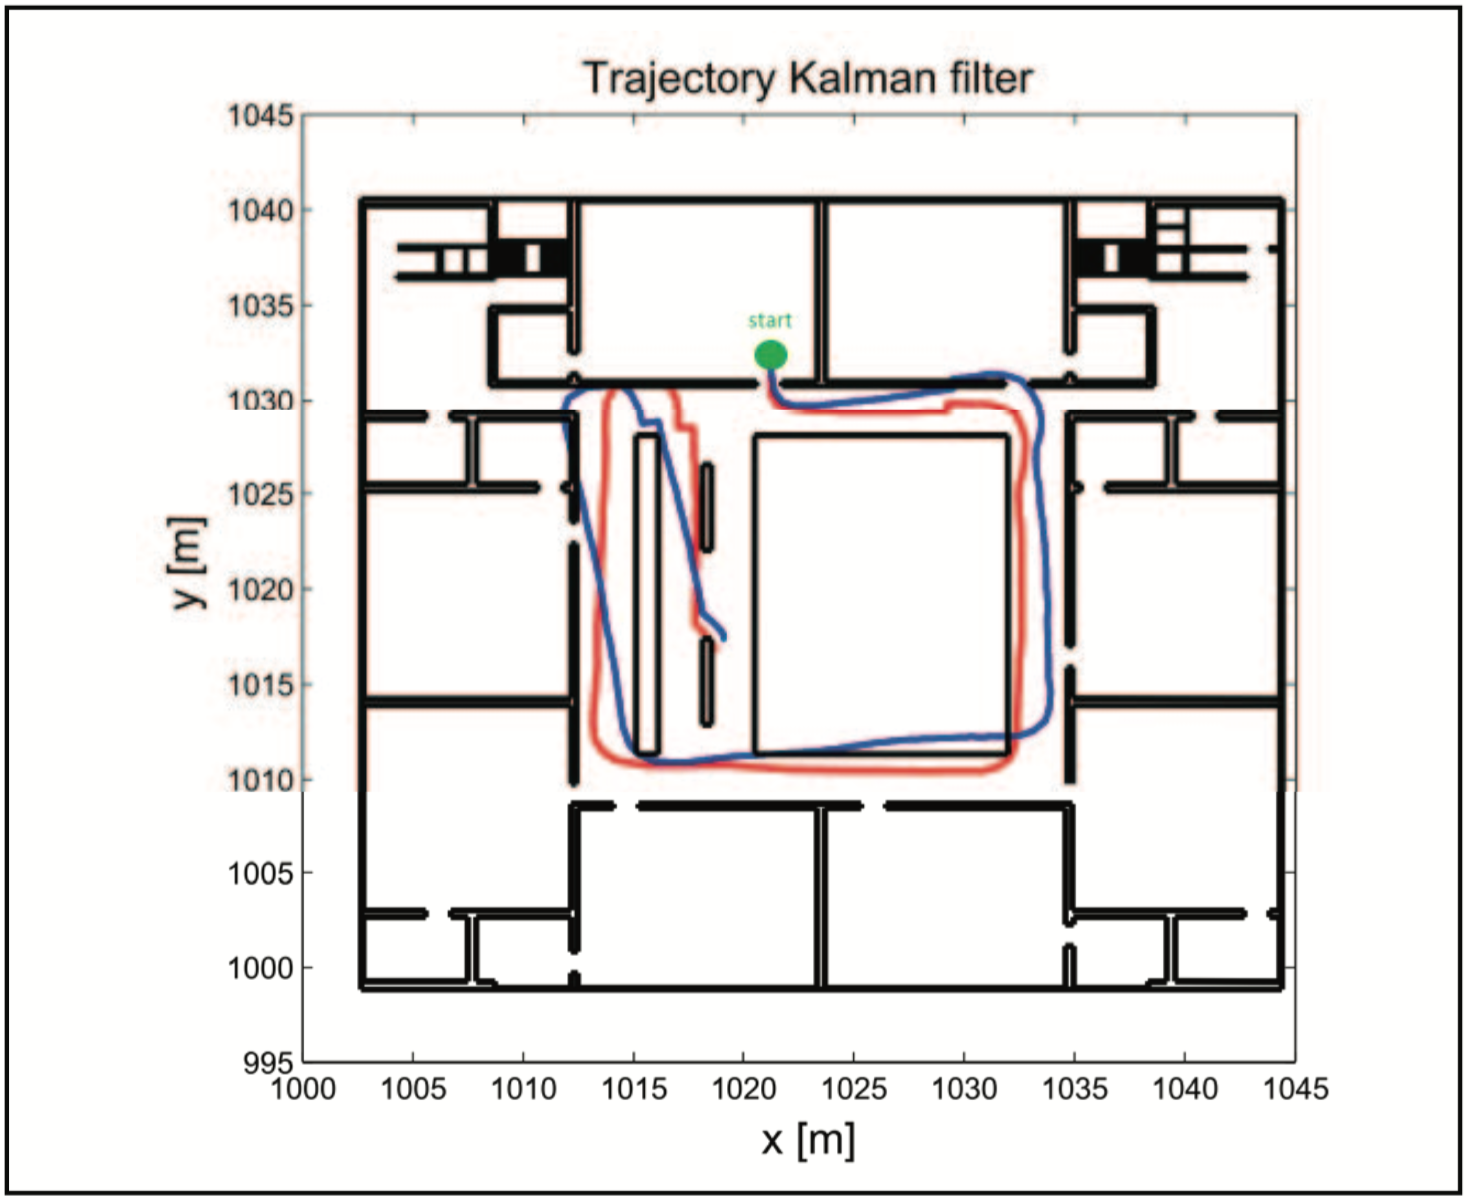
\includegraphics[width=150px]{img/pozition_estimation_with_kalman_filter.png}\label{fig:pozition_estimation_with_parctile_filter_a}}
    \subfloat[b][]{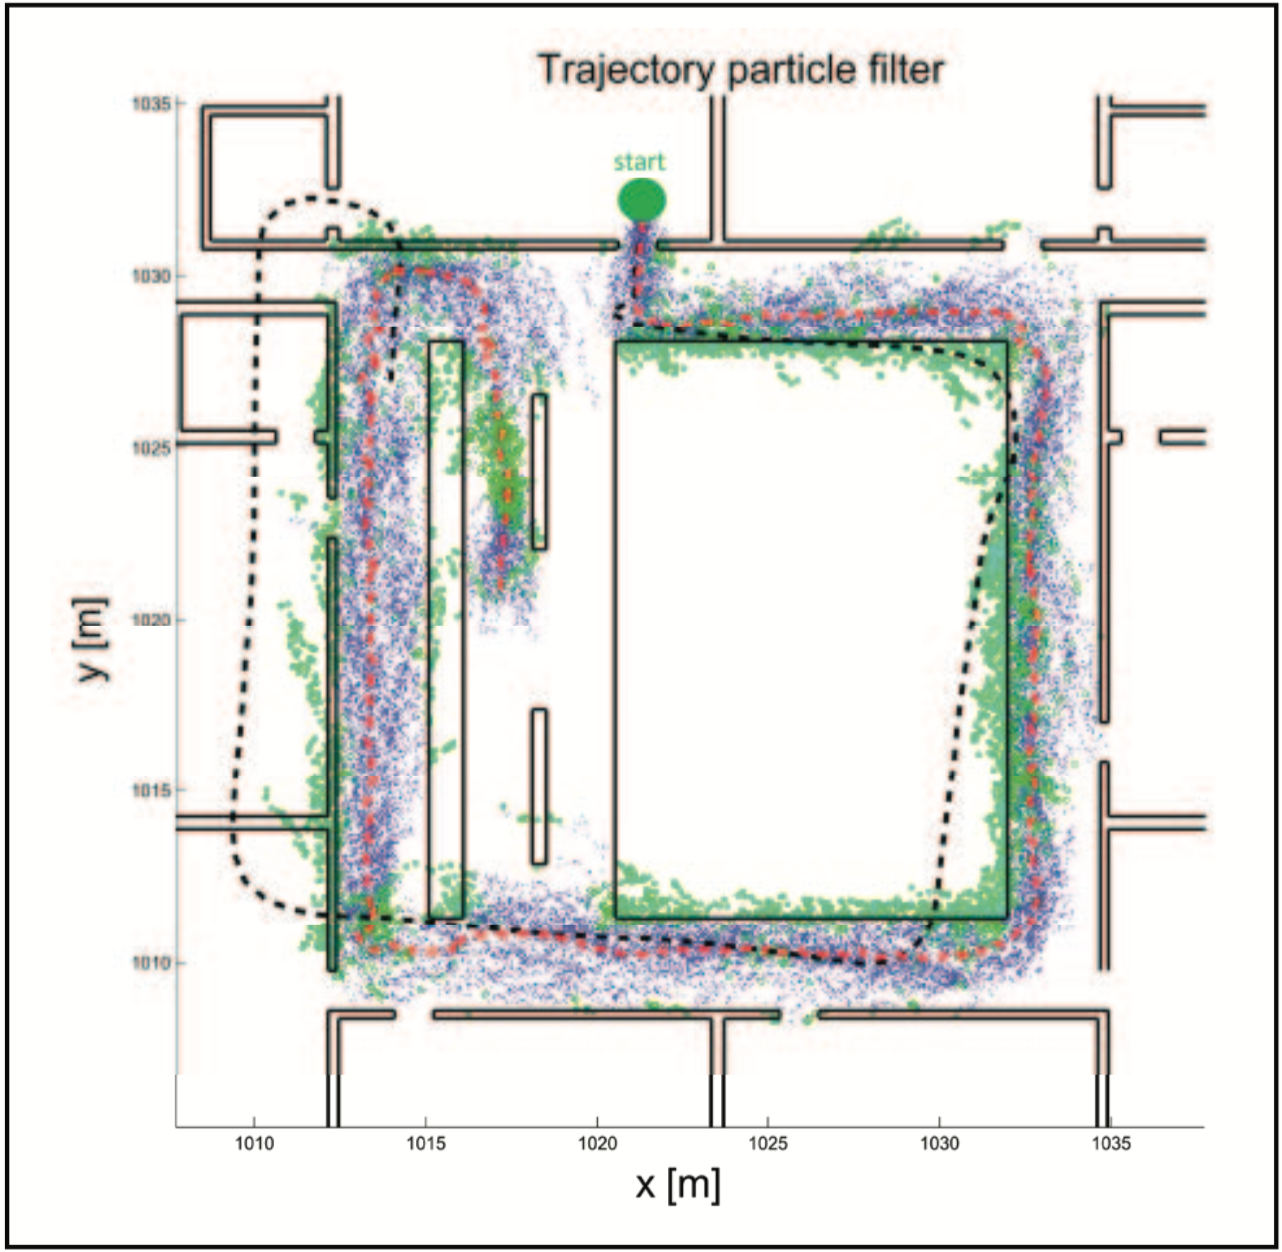
\includegraphics[width=150px]{img/pozition_estimation_with_particle_filter.png}\label{fig:pozition_estimation_with_parctile_filter_b}}
    \caption{Pozicijos filtravimas (a) dalelių ir (b) kalman filtru \cite{willemsenconcept}.}
\end{figure}


Tolimesniam darbe yra apžvelgiamos papildomos galimybės remti objekto pozicijos nustatymą, pavyzdžiui WiFi, magnetiniu lauku ar optinėmis sistemomis. Šio darbo tikslas nėra tokių sistemų nagrinėjimas, todėl tolimesnis darbo analizavimas yra stabdomas.

Darbo tikslas yra parodyti galima sistemos konstrukcija, kurios pagalba galima sukonstruoti pastato vidaus pozicijos nustatymo sistema, naudojant mobilų telefoną. Žemėlapio ir jutiklių kombinacija vektoriuje suteikia galimybę savarankiškai nustatyti dabartinę poziciją ir yra nepriklausoma nuo esamos pastato infrastruktūros ir pačios konstrukcijos ypatybės. Pozicijos nustatymas panaudojus Kalman arba dalelių filtrą yra įmanomas.  

\subsection{Dirbtinės žuvies pozicijos nustatymas}

Antras darbas apžvalgai yra pozicijos nustatymo sistema, nagrinėjanti povandeninių objektų pozicijos nustatymo atvejį \cite{yoo2011fuzzy}, ``Fuzzy logic based 2D position estimation for small robotic fish using low cost MEMS accelerometer''. Darbe yra pasiūloma efektyvi kalibravimo metodika ir dviejų dimensijų pozicijos nustatymo algoritmas, kuris yra paremtas raiškios logikos metodika. 

Pradedama nuo jutiklio klaidos modelio. Iš jutiklio nuskaitytą vertę galima išskaidyti į pilną vertę sudarančias komponentes. Dažniausiai vertė yra užrašoma tokia forma:

\begin{equation}
    a_{m,i} = a_{t,i} + B_i + S_{i}a_{t,i} + N_a{t,j} + \epsilon_i,
\end{equation}
kur $a_{m,j}$ yra pagreičio vertę $j$ ašyje, $a_t$ yra tikrasis pagreitis ašyje, $B$ yra įrangos pagreičio dedamoji, $S$ yra klaidos matricos santykio dydis, $N$ yra ne statmena matrica, o $\epsilon$ yra atsitiktinis triukšmas. Dedamoji, santykis ir ne statmena matrica yra pagrindiniai deterministiniai įverčiai šioje lygtyje. Jeigu šitos klaidos yra sumažinamos, tuomet liekamosios vertės bus labai mažos ir to pasekoje bus labai mažas sistemos dreifas. Kalibracijos procesas sprendžia šitą problemą, todėl labai svarbu atlikti šitą procesą prieš atliekant navigacinius matavimus. Pigioms ir praktinėms reikmėms, paprastas ir patikimas kalibracijos metodas yra labai reikalingas.

Kalibravimo procedūra susideda iš įrenginio išėjimo palyginimo su žinoma verte. Taip galima įvertinti išėjimo kokybę. Nuolatinės pozicijos šešių ašių kalibravimo metodika yra vertinama kaip dažniausiai naudojama metodika \cite{syed2007new}. Metodikos kokybė priklauso nuo to, kaip gerai įrenginio ašys yra sulygiuotos su vietinio kalibravimo įrenginio ašimis. Tokia procedūra gali sėkmingai nustatyti nuolatinę dedamąja ir santykio įvertį, tačiau nėra įmanoma įvertinti ne statmenumą. Darbas siūlo pagerinti šešių ašių kalibravimo metodiką 

\begin{equation}
    G = \tilde{M} \tilde{A}
\end{equation}
kur $G$ yra pagreičio jutiklio matavimo vektorius, $\tilde{M}$ yra ne statmenos matricos įverčiai kartu su santykio faktoriumi, o $\tilde{A}$ yra tikra pagreičio įverčių vektorius. Praleidžiant išvedimą, kuris yra pateikiamas darbe, ne statmenos matricos įverčiai yra randami

\begin{equation}
    \tilde{M} = G \cdot \tilde{A}^T \cdot (\tilde{A}\tilde{A}^T)^{-1}
\end{equation}

Taip ir randami kalibravimo parametrai, kurie užtikrina ne statmenos matricos parametrų apskaičiavimą.




